\documentclass[conference]{IEEEtran}
\IEEEoverridecommandlockouts
% The preceding line is only needed to identify funding in the first footnote. If that is unneeded, please comment it out.
%Template version as of 6/27/2024

\usepackage{cite}
\usepackage{amsmath,amssymb,amsfonts}
\usepackage{algorithmic}
\usepackage{graphicx}
\usepackage{textcomp}
\usepackage{xcolor}
% added for Sections IV and V
\usepackage{booktabs}
\usepackage{tikz}
\usetikzlibrary{arrows.meta,positioning,calc}
\usepackage{pgfplots}
\pgfplotsset{compat=1.18}
\usepgfplotslibrary{groupplots}
\def\BibTeX{{\rm B\kern-.05em{\sc i\kern-.025em b}\kern-.08em
    T\kern-.1667em\lower.7ex\hbox{\sc e}\kern-.125em\lower.7ex\hbox{\sc x}}}
\begin{document}

\title{Modeling Terrain-Vehicle Interaction for Off-Road Mobility Assessment}

\author{\IEEEauthorblockN{1\textsuperscript{st} Given Name Surname}
\IEEEauthorblockA{\textit{Department of Engineering Sciences} \\
\textit{ABV-IIITM Gwalior, India}\\
@iiitm.ac.in}
\and
\IEEEauthorblockN{2\textsuperscript{nd} Given Name Surname}
\IEEEauthorblockA{\textit{Department of Engineering Sciences} \\
\textit{ABV-IIITM Gwalior, India}\\
@iiitm.ac.in}
\and
\IEEEauthorblockN{3\textsuperscript{rd} Given Name Surname}
\IEEEauthorblockA{\textit{Department of Engineering Sciences} \\
\textit{ABV-IIITM Gwalior, India}\\
@iiitm.ac.in}
}

\maketitle

\begin{abstract}
Varshith and Shreyas
\end{abstract}

\begin{IEEEkeywords}
Terrain-Vehicle, Off-road mobility, ML
\end{IEEEkeywords}

\section{Introduction}

\section{Related Works}

\section{Problem Statement}

%%%%%%%%%%%%%%%%%%%%%%%%%%%%%%%%%%%%%%%%%%%%%%%%%%%%%%%%%%%%%%%%%%%%%%%%%%%%%%%%%%%%%%%%%%%%%%%%%
\section{Proposed Approach}
\label{sec:approach}

The proposed framework models terrain--vehicle interaction as a comparison between the rating
cone index (RCI) of the soil and the vehicle cone index (VCI) of each vehicle, both in psi.
Since soil strength changes from day to day, the framework forecasts RCI from a local weather
log and plans routes for the day of travel rather than the day of planning (shown in
Fig.~\ref{fig:framework}).

\subsection{Terrain--Vehicle Interaction Model}

\subsubsection{Soil Strength}
With the surface (0--7\,cm) and root-zone (7--28\,cm) soil moisture scaled to
$s^{(1)}_t, s^{(2)}_t \in [0,1]$, and $R^{3d}_t$ the rainfall of the last three days, the soil
wetness index (SWI) and soil strength on day $t$ are:
\begin{gather}
  \mathrm{SWI}_t = 0.35\,s^{(1)}_t + 0.65\,s^{(2)}_t , \\
  \mathrm{RCI}_t = 300\,e^{-k\,\mathrm{SWI}_t}
  \left(1 - 0.15\min\!\left(R^{3d}_t / 50\,\mathrm{mm},\ 1\right)\right),
  \label{eq:rci}
\end{gather}
where $k = \ln(300/15)$. As in the strength--moisture model used in~\cite{liu2025},
$\ln\mathrm{RCI}$ falls linearly with a moisture term, here the SWI. The constants are ours: an
assumed air-dry strength of 300, a saturated strength of 15 from field readings at
immobilisation~\cite{rosca2018}, layer weights spanning the NRMM critical layers of 0--15 and
15--30\,cm~\cite{haley1979}, and a rain factor of up to 15\% for surface water that daily soil
moisture misses.

\subsubsection{Vehicle Cone Index}
Each vehicle is characterised by its Mobility Index (MI)~\cite{rula1971,haley1979}. For a
tracked vehicle:
\begin{equation}
  \mathrm{MI} = \left(\frac{\mathrm{CPF}\cdot\mathrm{WF}}{\mathrm{TF}\cdot\mathrm{GF}}
  + \mathrm{BF} - \mathrm{CF}\right)\mathrm{EF}\cdot\mathrm{TrF},
\end{equation}
where CPF, WF, TF, GF, BF, CF, EF and TrF are the contact pressure, weight, track, grouser,
bogie, clearance, engine and transmission factors. MI gives the soil strength needed for one
pass and for 50 passes in the same track~\cite{ciobotaru2009}:
\begin{align}
  \mathrm{VCI}_1    &= 7.0 + 0.2\,\mathrm{MI} - 39.2/(\mathrm{MI} + 5.6), \\
  \mathrm{VCI}_{50} &= 19.27 + 0.43\,\mathrm{MI} - 125.79/(\mathrm{MI} + 7.08).
\end{align}
Wheeled vehicles use the corresponding wheeled forms~\cite{rosca2018}. Our implementation
reproduces the published M1 example (MI 98.6, $\mathrm{VCI}_1$ 26.3)~\cite{ciobotaru2009}.

\subsubsection{Interaction}
A vehicle is NO-GO when $\mathrm{RCI} < \mathrm{VCI}_1$, SLOW-GO when
$\mathrm{VCI}_1 \le \mathrm{RCI} < \mathrm{VCI}_{50}$, and GO otherwise~\cite{rula1971,rosca2018}.
SLOW-GO is quantified by the number of vehicles one track can carry:
\begin{equation}
  n(\mathrm{RCI}) = 50^{(\mathrm{RCI} - \mathrm{VCI}_1)/(\mathrm{VCI}_{50} - \mathrm{VCI}_1)},
  \label{eq:passes}
\end{equation}
and by its speed. Equation (\ref{eq:passes}) is ours: the sources give only the 1-pass and
50-pass requirements~\cite{rula1971}, so the required strength is taken to rise with $\ln n$
between them, giving 1 pass at $\mathrm{VCI}_1$ and 50 at $\mathrm{VCI}_{50}$.

The speed follows the fine-grained soil relations of the NATO Reference Mobility Model
(NRMM)~\cite{haley1979}, in which the motion resistance $R/W$, traction $T/W$ and slip $s$ of
the running gear are functions of the excess strength $\mathrm{RCI} - \mathrm{VCI}_1$. On a
slope $\theta$, the vehicle is stuck if $(T/W)\cos\theta < \sin\theta + (R/W)\cos\theta$;
otherwise its speed is where the rim pull meets the resistance:
\begin{equation}
  v = \min\!\left(\frac{\eta P\,(1 - s)}{W\left(\sin\theta + (R/W)\cos\theta\right)},\ v_{\max}\right),
  \label{eq:speed}
\end{equation}
where $P$ is the engine power, $W$ the weight, $v_{\max}$ the top speed and $\eta = 0.8$ an
assumed driveline efficiency. The constant-power rim pull $\eta P / v$ is ours, as NRMM builds
it gear by gear from engine data that the vehicle table lacks. On paved roads, the NRMM
hard-surface resistance replaces the soil terms.

\subsection{GRU--Ridge Forecaster}
The forecaster uses only the local weather log, without numerical weather prediction. As RCI
has a lag-1 autocorrelation of 0.99, it predicts the change in RCI for lead time
$h = 1, \dots, 7$ days:
\begin{equation}
  \widehat{\mathrm{RCI}}_{t+h} = \mathrm{RCI}_t
  + \tfrac{1}{2}\left[\bar g_h(\mathbf{X}_{t-59:t}) + r_h(\boldsymbol{\phi}_t)\right],
  \label{eq:forecast}
\end{equation}
where $\bar g_h$ is the mean of three gated recurrent unit (GRU) networks~\cite{cho2014}
(2 layers, 128 hidden units) over a 60-day input window $\mathbf{X}$, and $r_h$ is a ridge
regression~\cite{hoerl1970} on 128 causal features $\boldsymbol{\phi}_t$ (lags, rolling
statistics and seasonal terms). Equation (\ref{eq:forecast}) is ours: predicting the change
makes persistence the zero-change forecast, and averaging a nonlinear sequence model with a
linear feature model lets their errors partly cancel.
A vehicle of band $b$ is called NO-GO when:
\begin{equation}
  \widehat{\mathrm{RCI}}_{t+h} - m_{b,h} < \mathrm{VCI}_1 ,
  \label{eq:decision}
\end{equation}
where $m_{b,h}$ is the smallest safety margin that catches 90\% of NO-GO days. This rule is
ours: subtracting a margin biases the call towards safety, and tuning it per band and lead time
fixes the miss rate for each vehicle class. The GRUs are
trained with AdamW optimizer, Batch Size: 128, Epochs: 300 with early stopping (patience 30),
Learning Rate: 0.001 with a one-cycle schedule, Weight Decay: 0.0001 and mean squared error
loss. The forecaster has 531,228 parameters.

\subsection{Trafficability Mapping}
The forecast is spread over a 90\,m terrain grid by the topographic wetness
index~\cite{beven1979}, which shifts the SWI of each cell by up to $\pm 0.2$ in~(\ref{eq:rci}).
The soil membership of a cell is 0 below $\mathrm{VCI}_1$ and rises from 0.25 to 1 at
$\mathrm{VCI}_{50}$. Both steps are ours: wetter hollows soften first, and the floor of 0.25
keeps SLOW-GO ground slow rather than forbidden. Slope and land-cover memberships follow the
tables of Liu et al.~\cite{liu2025} for tracked and wheeled vehicles, with forest split into
sparse, open and dense canopy by NDVI; water is 0, and roads are 1 for both. The memberships
combine by fuzzy AND~\cite{zadeh1965}, which vetoes any
cell with a single impassable factor, as the improved map of~\cite{liu2025} does:
\begin{equation}
  \mu_c = \min\left(\mu^{\mathrm{slope}}_c,\ \mu^{\mathrm{cover}}_c,\ \mu^{\mathrm{soil}}_c\right).
  \label{eq:fuzzy}
\end{equation}
\subsection{Route Planning}
The map is converted to a graph in which each cell is linked to its eight neighbours, and NO-GO
cells ($\mu_c = 0$) are removed. The cost of the edge between cells $u$ and $v$ is the time to
cross it at a speed proportional to the membership:
\begin{equation}
  w(u,v) = d_{uv} \cdot \tfrac{1}{2}\left(1/\mu_u + 1/\mu_v\right),
  \label{eq:cost}
\end{equation}
where $d_{uv}$ is 90\,m, or $90\sqrt{2}$\,m on a diagonal. Equation (\ref{eq:cost}) is ours: each
half of a step is charged at the speed of the cell it lies in. Paved roads ignore soil
($\mu^{\mathrm{soil}} = 1$), while unpaved tracks soften like the ground around them. A trip
planned on day $t$ for day $t+h$ proceeds as follows:
\begin{enumerate}
  \item[1)] forecast $\widehat{\mathrm{RCI}}_{t+h}$ with (\ref{eq:forecast}) and subtract $m_{b,h}$;
  \item[2)] compute $\mu_c$ for every cell with (\ref{eq:fuzzy});
  \item[3)] build the graph with (\ref{eq:cost}) and find the least-cost route from the start
  with Dijkstra's algorithm~\cite{dijkstra1959};
  \item[4)] if no route reaches the destination, hold the trip back rather than send it over
  NO-GO ground.
\end{enumerate}
Dijkstra's algorithm finds routes of the same cost as the A* search of~\cite{liu2025} with an
admissible heuristic~\cite{hart1968}, and one search from a start serves every destination. For
travel-time routing, $1/\mu$ in (\ref{eq:cost}) is replaced by the time per km at the speed
of~(\ref{eq:speed}), scaled by the land-cover membership off road.

In a convoy, each pass weakens the track; inverting (\ref{eq:passes}), the $n$-th vehicle needs:
\begin{equation}
  \mathrm{VCI}(n) = \mathrm{VCI}_1 + (\mathrm{VCI}_{50} - \mathrm{VCI}_1)\ln n / \ln 50 ,
\end{equation}
which is ours and follows directly from~(\ref{eq:passes}). The vehicles plan in turn: after
each route, the pass count of its cells rises by one, and the next vehicle plans on the
updated map with $\mathrm{VCI}(n)$ in place of $\mathrm{VCI}_1$.

\begin{figure}[t]
  \centering
  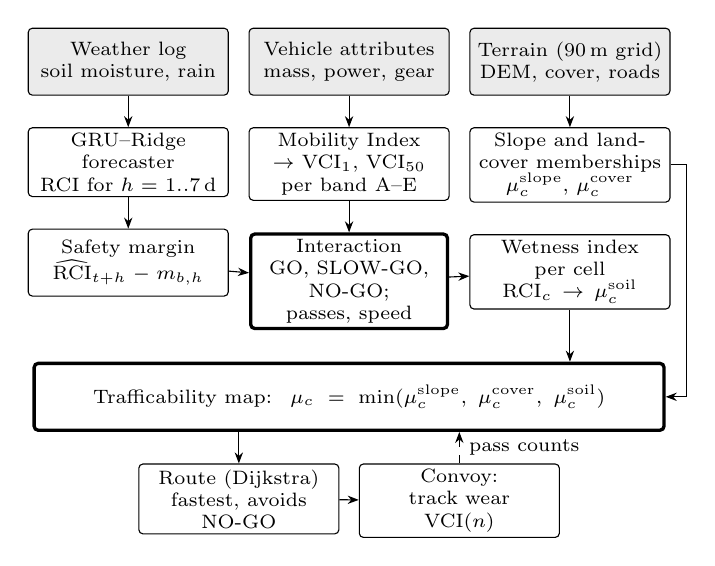
\begin{tikzpicture}[
      font=\scriptsize, >={Stealth[length=4pt]}, node distance=4mm and 2.5mm,
      box/.style={draw, rounded corners=1.5pt, align=center, minimum width=25mm,
                  text width=24mm, minimum height=8.5mm, inner sep=2pt, fill=white},
      data/.style={box, fill=black!8},
      key/.style={box, very thick}]
    \node[data] (wx)  {Weather log\\soil moisture, rain};
    \node[data, right=of wx] (veh) {Vehicle attributes\\mass, power, gear};
    \node[data, right=of veh] (ter) {Terrain (90\,m grid)\\DEM, cover, roads};
    \node[box, below=of wx]  (fc)  {GRU--Ridge\\forecaster\\RCI for $h = 1..7$\,d};
    \node[box, below=of veh] (mi)  {Mobility Index\\$\to$ VCI$_1$, VCI$_{50}$\\per band A--E};
    \node[box, below=of ter] (mem) {Slope and land-\\cover memberships\\$\mu^{\mathrm{slope}}_c$, $\mu^{\mathrm{cover}}_c$};
    \node[box, below=of fc]  (mar) {Safety margin\\$\widehat{\mathrm{RCI}}_{t+h} - m_{b,h}$};
    \node[key, below=of mi, text width=23mm] (int) {Interaction\\GO, SLOW-GO,\\NO-GO; passes, speed};
    \node[box, below=of mem] (twi) {Wetness index\\per cell\\$\mathrm{RCI}_c \to \mu^{\mathrm{soil}}_c$};
    \node[key, below=of int, minimum width=80mm, text width=78mm] (map)
         {Trafficability map: \ $\mu_c = \min(\mu^{\mathrm{slope}}_c,\ \mu^{\mathrm{cover}}_c,\ \mu^{\mathrm{soil}}_c)$};
    \node[box, below=of map, xshift=-14mm] (rt) {Route (Dijkstra)\\fastest, avoids NO-GO};
    \node[box, below=of map, xshift=14mm]  (cv) {Convoy: track wear\\$\mathrm{VCI}(n)$};
    \draw[->] (wx) -- (fc);
    \draw[->] (veh) -- (mi);
    \draw[->] (ter) -- (mem);
    \draw[->] (fc) -- (mar);
    \draw[->] (mi) -- (int);
    \draw[->] (mar) -- (int);
    \draw[->] (int) -- (twi);
    \draw[->] (twi) -- (twi |- map.north);
    \draw[->] (mem.east) -- ++(2mm,0) |- (map.east);
    \draw[->] (rt |- map.south) -- (rt);
    \draw[->] (rt) -- (cv);
    \draw[->, dashed] (cv) -- node[right] {pass counts} (cv |- map.south);
  \end{tikzpicture}
  \caption{Block diagram of the proposed framework. The forecaster predicts soil strength from
  the weather log, the Mobility Index gives each vehicle's cone indices, and the planner
  combines both with static terrain into a per-vehicle trafficability map and route.}
  \label{fig:framework}
\end{figure}

%%%%%%%%%%%%%%%%%%%%%%%%%%%%%%%%%%%%%%%%%%%%%%%%%%%%%%%%%%%%%%%%%%%%%%%%%%%%%%%%%%%%%%%%%%%%%%%%%
\section{Experimental Discussions}
\label{sec:experiments}

\subsection{Dataset Description}
In this study, the following three datasets are utilized:
\begin{enumerate}
  \item \emph{Pachmarhi Weather Record:} daily data for the Pachmarhi plateau (Satpura range,
  1,067\,m) from 2015 to 2025 (4,018 days), with two-layer soil moisture from the ERA5-Land
  reanalysis~\cite{munoz2021} and IMD gridded rainfall~\cite{pai2014} (ERA5 for 2025). RCI is
  derived with~(\ref{eq:rci}); it falls through the vehicle thresholds every monsoon
  (Fig.~\ref{fig:rci}).
  \item \emph{Vehicle Attribute Dataset:} a public list of 2,451 records compiled from a
  simulation game's files, of which mass and engine power are used. After cleaning, 1,145
  ground vehicles remain (1,004 tracked, 125 wheeled, 16 half-tracks); the running gear is
  read from the vehicle names, and track or tyre dimensions are assumed by weight class. As masses are
  per-template values, results are reported for five $\mathrm{VCI}_1$ bands (A: $<$18,
  B: 18--21, C: 21--24, D: 24--30, E: $\geq$30 psi), each planned with its median vehicle.
  \item \emph{Terrain Data:} a Google Earth Engine export with a 30\,m elevation model,
  ESA WorldCover~\cite{zanaga2022} and Sentinel-2 NDVI, aggregated to a 90\,m grid of 76,218
  cells, and 403 OpenStreetMap road segments~\cite{osm}.
\end{enumerate}
The record is split chronologically into Training (2015--21), Validation (2022--23) and
Testing (2024--25), with 2,498, 730 and 724 forecast origins. The safety margins are tuned on
one test year and scored on the other, in both directions.

\begin{figure}[t]
  \centering
  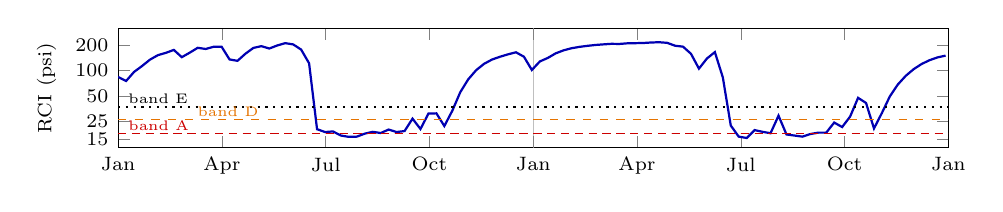
\begin{tikzpicture}
    \begin{axis}[
        width=\columnwidth, height=3.1cm, ymode=log, ymin=12, ymax=320,
        xmin=0, xmax=24, xtick={0,3,...,24},
        xticklabels={Jan,Apr,Jul,Oct,Jan,Apr,Jul,Oct,Jan},
        ytick={15,25,50,100,200}, yticklabels={15,25,50,100,200},
        ylabel={RCI (psi)}, ylabel style={font=\scriptsize}, tick label style={font=\scriptsize},
        extra x ticks={12}, extra x tick labels={}, extra x tick style={grid=major}]
      \addplot[thick, blue!70!black] coordinates {(0.00,84.0) (0.23,75.1) (0.46,96.4) (0.69,113.2) (0.92,135.0) (1.15,152.8) (1.38,162.8) (1.61,176.4) (1.84,144.4) (2.07,163.6) (2.30,186.9) (2.53,181.0) (2.76,192.3) (2.99,192.8) (3.22,135.8) (3.45,130.7) (3.68,158.9) (3.91,186.4) (4.14,195.6) (4.37,183.3) (4.60,199.3) (4.83,212.4) (5.06,205.2) (5.29,178.0) (5.52,122.2) (5.75,20.0) (5.98,18.5) (6.21,18.8) (6.44,16.8) (6.67,16.2) (6.90,16.3) (7.13,17.7) (7.36,18.6) (7.59,18.0) (7.82,19.8) (8.05,18.5) (8.28,19.0) (8.51,26.7) (8.74,20.1) (8.97,30.7) (9.20,30.9) (9.43,21.8) (9.66,33.2) (9.89,55.2) (10.12,78.6) (10.35,101.2) (10.58,120.5) (10.81,135.5) (11.04,146.3) (11.27,156.2) (11.50,165.3) (11.73,146.4) (11.96,101.6) (12.19,128.5) (12.42,141.5) (12.65,160.6) (12.88,174.5) (13.11,184.9) (13.34,191.9) (13.57,197.4) (13.80,202.1) (14.03,205.4) (14.26,208.5) (14.49,207.8) (14.72,211.4) (14.95,212.3) (15.18,213.3) (15.41,216.2) (15.64,217.8) (15.87,214.2) (16.10,197.9) (16.33,192.9) (16.56,158.5) (16.79,105.5) (17.02,139.2) (17.25,166.1) (17.48,83.0) (17.71,22.1) (17.94,16.3) (18.17,15.7) (18.40,19.5) (18.63,18.6) (18.86,17.9) (19.09,29.0) (19.32,17.3) (19.55,16.8) (19.78,16.3) (20.01,17.5) (20.24,18.2) (20.47,18.2) (20.70,24.0) (20.93,21.2) (21.16,28.3) (21.39,47.3) (21.62,41.1) (21.85,20.4) (22.08,31.3) (22.31,49.4) (22.54,68.3) (22.77,86.7) (23.00,104.2) (23.23,120.0) (23.46,133.2) (23.69,143.8) (23.92,150.8)};
      \addplot[densely dashed, red!80!black, domain=0:24] {17.6};
      \addplot[dashed, orange!90!black, domain=0:24] {26.2};
      \addplot[dotted, thick, black, domain=0:24] {36.7};
      \node[font=\tiny, red!80!black, anchor=south west, inner sep=1pt] at (axis cs:0.2,17.6) {band A};
      \node[font=\tiny, orange!90!black, anchor=south west, inner sep=1pt] at (axis cs:2.2,26.2) {band D};
      \node[font=\tiny, anchor=south west, inner sep=1pt] at (axis cs:0.2,36.7) {band E};
    \end{axis}
  \end{tikzpicture}
  \caption{Weekly mean soil strength over the 2024--25 test years against the one-pass cone
  index $\mathrm{VCI}_1$ of bands A (light tracked), D (heavy tracked) and E (wheeled). Below a
  line, that band is NO-GO.}
  \label{fig:rci}
\end{figure}

\subsection{Classification Performance Metrics}
Each trafficability call is a binary classification of a vehicle-day, with NO-GO as the
positive class, giving True Positives (TP), False Negatives (FN), False Positives (FP) and
True Negatives (TN). The following metrics are employed:
\begin{enumerate}
  \item[a)] \emph{Recall:} $\mathrm{TP}/(\mathrm{TP} + \mathrm{FN})$
  \item[b)] \emph{Precision:} $\mathrm{TP}/(\mathrm{TP} + \mathrm{FP})$
  \item[c)] \emph{False NO-GO calls:} FP per vehicle-year
  \item[d)] \emph{$R^2$:} $1 - \sum(y - \hat y)^2 / \sum(y - \bar y)^2$
\end{enumerate}
As the margin~(\ref{eq:decision}) is tuned to 90\% recall, decisions are compared on false
NO-GO calls at equal recall. A planned trip is \emph{stuck} if its route crosses a NO-GO cell
on the travel day, and \emph{held} if no route is planned although one existed.

\subsection{Experimental Results}

\subsubsection{Model Selection}
Ten forecasting models were tested on the same inputs and years (Table~\ref{tab:arch}), with
the deep models averaged over three seeds. The GRU--Ridge
forecaster has the second-lowest RMSE averaged over the seven lead times (14.64\,psi) and the
fewest false NO-GO calls of the deep models at 7 days, with fewer parameters than the TFT and
N-BEATS, so it is used in the rest of the evaluation.

\begin{table}[t]
  \caption{Forecasting models tested on the 2024--25 test years: RMSE (psi) by lead time, and
  false NO-GO calls per vehicle-year (FP/yr) at 90\% recall. Parameters count all three seeds.}
  \label{tab:arch}
  \centering
  \footnotesize
  \setlength{\tabcolsep}{3pt}
  \begin{tabular}{@{}lrrrrrr@{}}
    \toprule
    & & \multicolumn{3}{c}{RMSE} & \multicolumn{2}{c}{FP/yr} \\
    \cmidrule(lr){3-5} \cmidrule(l){6-7}
    Model & Params & 1 d & 3 d & 7 d & 3 d & 7 d \\
    \midrule
    Persistence                          & --     & 6.71 & 15.16 & 26.02 & 30.4 & 45.8 \\
    Climatology                          & --     & 35.60 & 35.47 & 34.73 & 23.4 & \textbf{23.4} \\
    ARIMAX~\cite{hyndman2021}            & 14     & \textbf{5.69} & 13.88 & 22.16 & 22.9 & 29.5 \\
    Random Forest~\cite{markova2025}     & --     & 6.55 & 14.93 & 23.89 & 25.4 & 32.7 \\
    LightGBM~\cite{ke2017}               & --     & 6.33 & 14.51 & 24.84 & 25.6 & 32.5 \\
    LSTM~\cite{wang2024hess}             & 690k   & 7.05 & 15.46 & 22.58 & 22.8 & 35.7 \\
    TCN~\cite{villia2022}                & 370k   & 5.84 & 13.66 & 22.89 & 23.1 & 35.7 \\
    Transformer~\cite{wang2024agwat}     & 1.85M  & 6.09 & 13.88 & 22.61 & \textbf{19.7} & 34.6 \\
    TFT~\cite{lim2021}                   & 3.47M  & 6.05 & \textbf{12.83} & 21.18 & 23.2 & 35.7 \\
    N-BEATS~\cite{oreshkin2020}          & 2.29M  & 6.15 & 13.50 & \textbf{20.68} & 24.1 & 32.4 \\
    \textbf{GRU--Ridge (ours)}           & 531k   & 6.05 & 13.29 & 20.76 & 24.0 & 31.4 \\
    \bottomrule
  \end{tabular}
\end{table}

\subsubsection{Comparison with Past Works}
Table~\ref{tab:past} compares the proposed framework with published results; as those works
use data from other sites, our forecasts are converted to their target, soil wetness, by
inverting~(\ref{eq:rci}). The proposed forecaster reaches $R^2$ of 0.991, 0.960 and 0.903 at
1, 3 and 7 days, higher at every lead time than all models of~\cite{wang2024hess}, including
their best (GAN-LSTM, 0.963, 0.919 and 0.846), and than the mean $R^2$ of 0.523
of~\cite{wang2024agwat}. It is also the only approach that forecasts soil strength days ahead,
assesses each vehicle and plans routes on the forecast; against the trafficability map of Liu
et al.~\cite{liu2025}, it sends 27\% fewer trips into mud at 7 days (Section~\ref{sec:res-route}).

\begin{table}[t]
  \caption{Comparison with past works. SM: soil moisture; CI: cone index; TM: trafficability
  map. $R^2$ of the proposed forecaster is on soil wetness, converted from its RCI forecast.}
  \label{tab:past}
  \centering
  \footnotesize
  \setlength{\tabcolsep}{2.6pt}
  \begin{tabular}{@{}llcccccc@{}}
    \toprule
    & & & & & \multicolumn{3}{c}{$R^2$} \\
    \cmidrule(l){6-8}
    Work & Model & Target & Vehicle & Route & 1 d & 3 d & 7 d \\
    \midrule
    \cite{liu2025}        & AHP map     & TM  & \checkmark & \checkmark & -- & -- & -- \\
    \cite{markova2025}    & RF          & CI  & $\times$   & $\times$   & -- & -- & -- \\
    \cite{wang2024hess}   & RF          & SM  & $\times$   & $\times$   & 0.929 & 0.891 & 0.832 \\
    \cite{wang2024hess}   & LSTM        & SM  & $\times$   & $\times$   & 0.963 & 0.916 & 0.842 \\
    \cite{wang2024hess}   & Transformer & SM  & $\times$   & $\times$   & 0.952 & 0.912 & 0.843 \\
    \cite{wang2024hess}   & GAN-LSTM    & SM  & $\times$   & $\times$   & 0.963 & 0.919 & 0.846 \\
    \cite{wang2024agwat}  & Transformer & SM  & $\times$   & $\times$   & \multicolumn{3}{c}{0.523 (mean)} \\
    \textbf{Ours} & \textbf{GRU--Ridge} & RCI & \checkmark & \checkmark & \textbf{0.991} & \textbf{0.960} & \textbf{0.903} \\
    \bottomrule
  \end{tabular}
\end{table}

\subsubsection{Results by Vehicle Band}
Table~\ref{tab:slowgo} gives, for each band's planning vehicle, the share of 2024--25 test days
that are NO-GO and SLOW-GO, the passes~(\ref{eq:passes}) and level-ground
speed~(\ref{eq:speed}) on its SLOW-GO days, and the false NO-GO calls at 7 days. A typical
SLOW-GO day lets only 2--5 vehicles use one track, at 14--32\,km/h against 57--60\,km/h on dry
ground; at 5\,psi above $\mathrm{VCI}_1$, one track carries 1.5--2.3 vehicles at 12--16\,km/h.
Against the same margin rule on persistence, the forecast makes 23--45\% fewer false NO-GO
calls at equal recall in every band. Light tracked vehicles (band A) are the hardest case, as
their $\mathrm{VCI}_1$ lies close to the saturated soil strength. Routing on the travel time
of~(\ref{eq:speed}) instead of on $\mu_c$ shortens trips by about 5\% at the same stuck rate,
and the travel time predicted at planning is on average within 0.3\% (3 days) and 1.0\%
(7 days) of the time on the travel day.

\begin{table}[t]
  \caption{Results by vehicle band on the 2024--25 test days: share of days NO-GO and SLOW-GO,
  median passes per track and level-ground speed on SLOW-GO days, and false NO-GO calls per
  vehicle-year at 7 days and 90\% recall for persistence (P) and the proposed forecaster (F).}
  \label{tab:slowgo}
  \centering
  \footnotesize
  \setlength{\tabcolsep}{2.2pt}
  \begin{tabular}{@{}lrrrrrrr@{}}
    \toprule
    & & & & \multicolumn{2}{c}{SLOW-GO days} & \multicolumn{2}{c}{FP/yr} \\
    \cmidrule(lr){5-6} \cmidrule(l){7-8}
    Band & VCI$_1$ & NO-GO & SLOW-GO & Passes & km/h & P & F \\
    \midrule
    A (tracked) & 17.6 & 13.3\% & 21.8\% & 1.8 & 14.2 & 74.0 & \textbf{54.3} \\
    B (tracked) & 19.0 & 18.9\% & 16.8\% & 2.4 & 13.9 & 54.0 & \textbf{34.0} \\
    C (tracked) & 21.6 & 24.4\% & 12.9\% & 2.7 & 13.8 & 43.9 & \textbf{27.8} \\
    D (tracked) & 26.2 & 29.0\% &  9.8\% & 3.4 & 18.6 & 28.6 & \textbf{22.0} \\
    E (wheeled) & 36.7 & 33.9\% &  8.6\% & 5.2 & 31.7 & 13.8 & \textbf{7.6} \\
    \bottomrule
  \end{tabular}
\end{table}

\subsubsection{Route Planning}
\label{sec:res-route}
Over 325,800 trips of 8--25\,km per planner (30 per test day, band and lead time), planning on
terrain alone sends 35.5\% of trips into mud. Planning on the forecast beats planning on today's
map~\cite{liu2025} on both errors: 1.6\% against 2.1\% of trips stuck at 3 days (24\% fewer)
and 2.9\% against 4.0\% at 7 days (27\% fewer), with fewer trips held back. A margin on today's
map is slightly safer at its tuned setting but holds back nearly twice as many trips. Sweeping both margins
(Fig.~\ref{fig:tradeoff}) shows that at an equal stuck rate the forecast holds back 40\%
(3 days) and 31\% (7 days) fewer trips. Without the veto of~(\ref{eq:fuzzy}), a weighted mean of
the same memberships sends 34.8\% of trips into mud.

\begin{figure}[t]
  \centering
  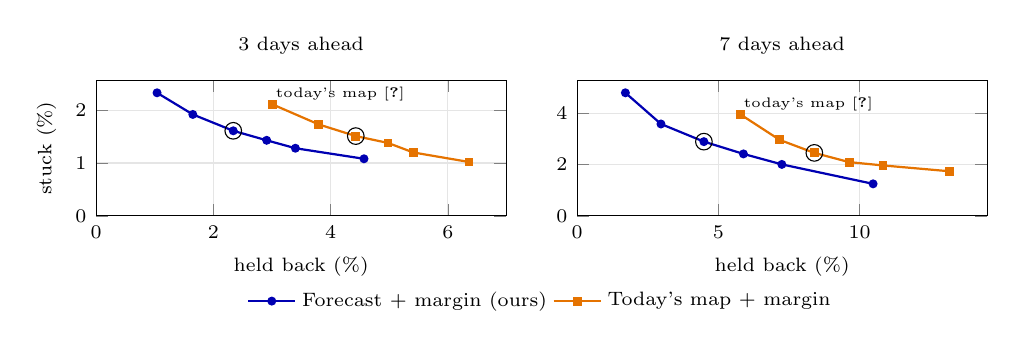
\begin{tikzpicture}
    \begin{groupplot}[
        group style={group size=2 by 1, horizontal sep=9mm},
        width=0.56\columnwidth, height=3.3cm,
        xlabel={held back (\%)}, xlabel style={font=\scriptsize},
        tick label style={font=\scriptsize}, title style={font=\scriptsize},
        ymin=0, xmin=0, grid=major, grid style={black!10}]
      \nextgroupplot[title={3 days ahead}, ylabel={stuck (\%)}, ylabel style={font=\scriptsize},
                     legend to name=tradeleg, legend columns=2, legend style={font=\scriptsize, draw=none}]
        \addplot[thick, blue!70!black, mark=*, mark size=1.2pt] coordinates
          {(1.04,2.33) (1.65,1.92) (2.34,1.61) (2.91,1.43) (3.40,1.28) (4.57,1.08)};
        \addlegendentry{Forecast + margin (ours)}
        \addplot[thick, orange!90!black, mark=square*, mark size=1.2pt] coordinates
          {(3.01,2.11) (3.80,1.73) (4.43,1.51) (4.98,1.38) (5.41,1.20) (6.36,1.02)};
        \addlegendentry{Today's map + margin}
        \addplot[only marks, mark=o, mark size=3pt, black] coordinates {(2.34,1.61) (4.43,1.51)};
        \node[font=\tiny, anchor=south west, inner sep=1pt] at (axis cs:3.01,2.11) {today's map~\cite{liu2025}};
      \nextgroupplot[title={7 days ahead}]
        \addplot[thick, blue!70!black, mark=*, mark size=1.2pt] coordinates
          {(1.71,4.81) (2.97,3.59) (4.49,2.90) (5.89,2.42) (7.25,2.01) (10.48,1.25)};
        \addplot[thick, orange!90!black, mark=square*, mark size=1.2pt] coordinates
          {(5.79,3.96) (7.17,2.97) (8.40,2.46) (9.63,2.10) (10.83,1.97) (13.20,1.74)};
        \addplot[only marks, mark=o, mark size=3pt, black] coordinates {(4.49,2.90) (8.40,2.46)};
        \node[font=\tiny, anchor=south west, inner sep=1pt] at (axis cs:5.79,3.96) {today's map~\cite{liu2025}};
    \end{groupplot}
    \node[below=7mm] at ($(group c1r1.south)!0.5!(group c2r1.south)$) {\pgfplotslegendfromname{tradeleg}};
  \end{tikzpicture}
  \caption{Routing backtest, 2024--25: trips sent into NO-GO ground (stuck) against possible
  trips held back, as each planner's safety margin is scaled from zero (today's map, no margin)
  to three times its tuned value (ringed). Lower left is better.}
  \label{fig:tradeoff}
\end{figure}

\subsubsection{Convoy Coordination}
On soft test days, a convoy of ten heavy tracked vehicles (band D) that follows the leader's
route gets 5.5 vehicles through on average, as the lead track fails under the vehicles behind.
Re-planning on the pass counts gets 9.2 through. Wheeled vehicles (band E) gain less (6.8 to
7.3), as the forest leaves them few parallel lanes.
%%%%%%%%%%%%%%%%%%%%%%%%%%%%%%%%%%%%%%%%%%%%%%%%%%%%%%%%%%%%%%%%%%%%%%%%%%%%%%%%%%%%%%%%%%%%%%%%%

\section{Conclusion}

\section*{Acknowledgment}

\begin{thebibliography}{00}
\bibitem{b1} G. Eason, B. Noble, and I. N. Sneddon, ``On certain integrals of Lipschitz-Hankel type involving products of Bessel functions,'' Phil. Trans. Roy. Soc. London, vol. A247, pp. 529--551, April 1955.
\bibitem{liu2025} Q. Liu, X. You, X. Zhang, and J. Zuo, ``Construction of dynamic trafficability map for unmanned vehicles considering multiple environmental factors and path planning,'' Scientific Reports, vol. 15, p. 9957, 2025.
\bibitem{rosca2018} P. Ro\c{s}ca, T. Ciobotaru, G. Olaru, and C. Puic\u{a}, ``Considerations regarding vehicle cone index for fine-grained soil,'' Journal of Military Technology, vol. 1, no. 2, pp. 39--44, 2018.
\bibitem{haley1979} P. W. Haley, M. P. Jurkat, and P. M. Brady, Jr., ``NATO reference mobility model, Edition I, users guide, volume I,'' U.S. Army Tank-Automotive Research and Development Command, Warren, MI, Tech. Rep. 12503, 1979.
\bibitem{rula1971} A. A. Rula and C. J. Nuttall, Jr., ``An analysis of ground mobility models (ANAMOB),'' U.S. Army Engineer Waterways Experiment Station, Vicksburg, MS, Tech. Rep. M-71-4, 1971.
\bibitem{ciobotaru2009} T. Ciobotaru, ``Semi-empiric algorithm for assessment of the vehicle mobility,'' Leonardo Electronic Journal of Practices and Technologies, vol. 8, no. 15, pp. 19--30, 2009.
\bibitem{cho2014} K. Cho, B. van Merri\"{e}nboer, C. Gulcehre, D. Bahdanau, F. Bougares, H. Schwenk, and Y. Bengio, ``Learning phrase representations using RNN encoder--decoder for statistical machine translation,'' in Proc. EMNLP, 2014, pp. 1724--1734.
\bibitem{hoerl1970} A. E. Hoerl and R. W. Kennard, ``Ridge regression: Biased estimation for nonorthogonal problems,'' Technometrics, vol. 12, no. 1, pp. 55--67, 1970.
\bibitem{beven1979} K. J. Beven and M. J. Kirkby, ``A physically based, variable contributing area model of basin hydrology,'' Hydrological Sciences Bulletin, vol. 24, no. 1, pp. 43--69, 1979.
\bibitem{zadeh1965} L. A. Zadeh, ``Fuzzy sets,'' Information and Control, vol. 8, no. 3, pp. 338--353, 1965.
\bibitem{dijkstra1959} E. W. Dijkstra, ``A note on two problems in connexion with graphs,'' Numerische Mathematik, vol. 1, pp. 269--271, 1959.
\bibitem{hart1968} P. E. Hart, N. J. Nilsson, and B. Raphael, ``A formal basis for the heuristic determination of minimum cost paths,'' IEEE Transactions on Systems Science and Cybernetics, vol. 4, no. 2, pp. 100--107, 1968.
\bibitem{munoz2021} J. Mu\~{n}oz-Sabater et al., ``ERA5-Land: A state-of-the-art global reanalysis dataset for land applications,'' Earth System Science Data, vol. 13, no. 9, pp. 4349--4383, 2021.
\bibitem{pai2014} D. S. Pai, L. Sridhar, M. Rajeevan, O. P. Sreejith, N. S. Satbhai, and B. Mukhopadhyay, ``Development of a new high spatial resolution ($0.25^\circ \times 0.25^\circ$) long period (1901--2010) daily gridded rainfall data set over India and its comparison with existing data sets over the region,'' Mausam, vol. 65, no. 1, pp. 1--18, 2014.
\bibitem{zanaga2022} D. Zanaga et al., ``ESA WorldCover 10 m 2021 v200,'' Zenodo, 2022, doi: 10.5281/zenodo.7254221.
\bibitem{osm} OpenStreetMap contributors, ``OpenStreetMap,'' 2026. [Online]. Available: https://www.openstreetmap.org
\bibitem{hyndman2021} R. J. Hyndman and G. Athanasopoulos, Forecasting: Principles and Practice, 3rd ed. Melbourne, Australia: OTexts, 2021.
\bibitem{markova2025} L. Markov\'{a}, D. Sl\'{a}dek, M. Hub\'{a}\v{c}ek, V. Talhofer, and P. Kol\'{a}\v{r}, ``Meteorological data-driven approach for soil passability modeling in GIS using machine learning,'' Geofizika, vol. 42, no. 1, 2025, doi: 10.15233/gfz.2025.42.4.
\bibitem{ke2017} G. Ke, Q. Meng, T. Finley, T. Wang, W. Chen, W. Ma, Q. Ye, and T.-Y. Liu, ``LightGBM: A highly efficient gradient boosting decision tree,'' in Proc. NeurIPS, 2017, pp. 3146--3154.
\bibitem{wang2024hess} Y. Wang, L. Shi, Y. Hu, X. Hu, W. Song, and L. Wang, ``A comprehensive study of deep learning for soil moisture prediction,'' Hydrology and Earth System Sciences, vol. 28, pp. 917--943, 2024.
\bibitem{villia2022} M. M. Villia, G. Tsagkatakis, M. Moghaddam, and P. Tsakalides, ``Embedded temporal convolutional networks for essential climate variables forecasting,'' Sensors, vol. 22, no. 5, p. 1851, 2022.
\bibitem{wang2024agwat} Y. Wang and Y. Zha, ``Comparison of transformer, LSTM and coupled algorithms for soil moisture prediction in shallow-groundwater-level areas with interpretability analysis,'' Agricultural Water Management, vol. 305, p. 109120, 2024.
\bibitem{lim2021} B. Lim, S. \"{O}. Ar\i{}k, N. Loeff, and T. Pfister, ``Temporal fusion transformers for interpretable multi-horizon time series forecasting,'' International Journal of Forecasting, vol. 37, no. 4, pp. 1748--1764, 2021.
\bibitem{oreshkin2020} B. N. Oreshkin, D. Carpov, N. Chapados, and Y. Bengio, ``N-BEATS: Neural basis expansion analysis for interpretable time series forecasting,'' in Proc. ICLR, 2020.
\end{thebibliography}

\end{document}
